% !TEX root = smc_bandits.tex
We evaluate the application of SMC-based policies in a real-life application of bandits:
the recommendation of personalized news articles, as previously done by \citet{ic-Chapelle2011}.
%Online content recommendation represents an important example of reinforcement learning, as it requires efficient balancing of the exploration and exploitation tradeoff.
%

We use a dataset\footnote{
	Available at \href{https://webscope.sandbox.yahoo.com/catalog.php?datatype=r\&did=49}{R6A - Yahoo! Front Page Today Module User Click Log Dataset.}
} that contains a fraction of user click logs for news articles displayed in the Featured Tab of the Today Module on the Yahoo! Front Page during the first ten days in May 2009. The articles to be displayed were originally chosen uniformly at random from a hand-picked pool of high-quality articles.
From these pool of original candidates,
we pick a subset of 20 articles shown at different times within May 6th,
and collect all user interactions logged with these articles,
for a total of 500,354 events.
In the dataset,
each user is associated with six features:
a bias term and 5 features that correspond to the membership features constructed via the conjoint analysis with a bilinear model described in~\citep{ip-Chu2009}.

The goal is to identify the most interesting article for each user,
or in bandit terms,
to maximize the total number of clicks on the recommended articles over all user interactions,
\ie the average click-through rate (CTR).

We treat each article as a bandit arm ($|\A|=20$),
and define whether the article is clicked or not by the user as a binary reward: $y_t=\{1,0\}$.
Hence, we pose the problem as a MAB with logistic rewards,
where we incorporate the user features as context, $x_t\in \Real^6$.

We implement SMC-based Thompson sampling only, due to the flexibility shown in simulated scenarios,
and its lack of hyperparameter tuning.

We argue that a news recommendation system should evolve over time,
as the relevance of news might change during the course of the day.
We evaluate both stationary and non-stationary bandits with logistic rewards.

As shown in Figure~\ref{fig:yahoo_logistic_dynamic},
we observe the flexibility of a non-stationary logistic bandit model,
where we notice how the SMC-based TS agent is able to pick up the dynamic popularity of certain articles over time
---averaged CTR results are provided in Table \ref{tab:yahoo_logistic_crt}.

% Figure
\begin{figure}[!h]
	\centering
	\vspace*{-2ex}
	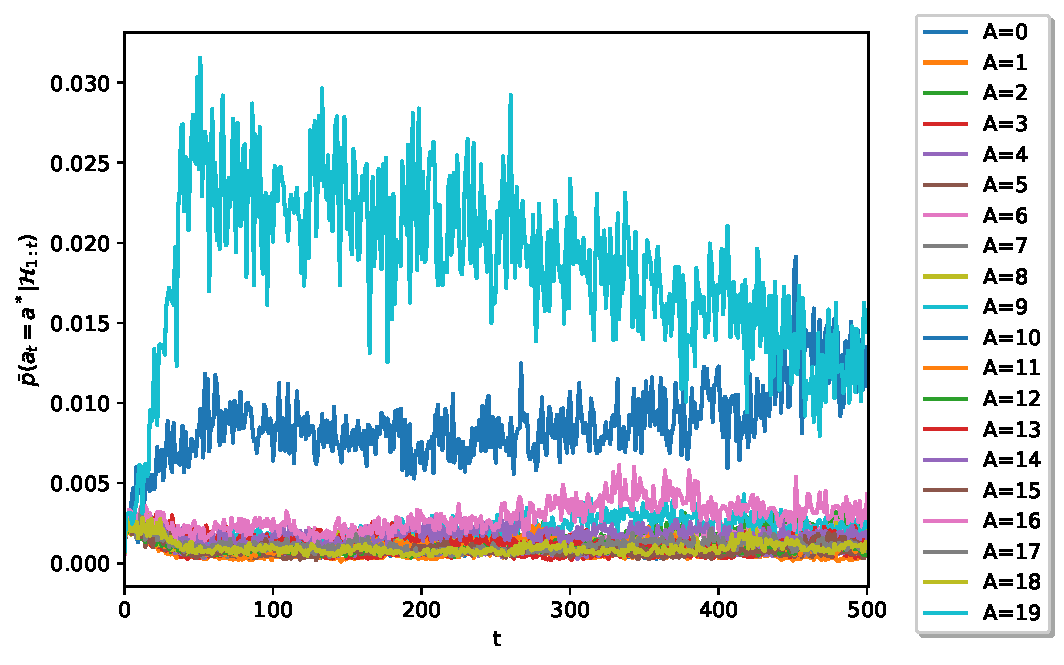
\includegraphics[width=0.85\textwidth]{./fods_figs/yahoo/yahoo_logistic_dynamic}
	\vspace*{-2ex}
	\caption{Empirical probability of playing each bandit arm over time, for SMC-based dynamic logistic Thompson sampling.
		The proposed dynamic bandit policy captures the changing popularity of articles over time.}
	\label{fig:yahoo_logistic_dynamic}
\end{figure}

% Table
%%%%%%%%%%%%%%%%%%%%%%%%
%% Table for yahoo data with logistic bandits
%%%%%%%%%%%%%%%%%%%%%%%%
\begin{table}[!ht]
	\begin{center}
		\resizebox*{\textwidth}{!}{
			\begin{tabular}{*{3}{|c}|}
				\hline
				% Header
				Model \cellcolor[gray]{0.6} & CTR\cellcolor[gray]{0.6} & Normalized CTR\cellcolor[gray]{0.6} \\ \hline
				% table starts
				\cellcolor[gray]{0.8} Logistic rewards, static arms & 0.0670 +/- 0.0088 & 1.6095 +/- 0.2115  \\ \hline
				\cellcolor[gray]{0.8} Logistic rewards, time-evolving arms & 0.0655 +/- 0.0082 & 1.5745 +/- 0.2064 \\ \hline
			\end{tabular}
		}
		\caption{CTR results for SMC-based policies on the news article recommendation dataset.
			The normalized CTR is with respect to a random recommendation baseline.}
		\label{tab:yahoo_logistic_crt}
	\end{center}
	\vspace*{-2ex}
\end{table}

